\chapter{Background and related work}
\label{chap:background}

\section{Deep Learning}

\section{Recommender systems}

\subsection{"Field-aware Factorization Machines for CTR Prediction", \citeyear{ffmctr} \cite{ffmctr}}

An effective method for classifying very large yet sparse data sets.

SOTA for several CTR-problems.

Has an over-fitting problem, but this can be mitigated by using early stopping.

\subsection{"Personalizing Session-based Recommendations with Hierarchical Recurrent Neural Networks", \citeyear{QuadranaKHC17} \cite{QuadranaKHC17}}

Simple matrix factorization does not take into account the timing and order of user events, and as a result are less responsiveness to changes in user behavior, e.g. new interests.

A \acrfull{rnn} can be used to exploit the timing and order of user events, but they may find it hard to model long sequences of user events over multiple sessions.

Because of this the \acrfull{hrnn} is introduced. It has two \acrfullpl{gru} instead of just one. One \acrshort{gru} models the session-level user activity, while another \acrshort{gru} models the user activity across sessions.

\subsection{"Temporal-Contextual Recommendation in Real-Time", \citeyear{tempcon} \cite{tempcon}}

2020. Introduces a black-box \acrshort{recsys} that can adapt to multiple use cases without the need for tuning. Achieves SOTA-performance on several data sets. Awarded best applied data science paper by SIGKDD for the 2020 digital conference.

Builds on the model described in \cite{QuadranaKHC17}, but improves on some aspects like efficiency, while still achieving comparable or even better results.

They also extended \acrshort{hrnn} by adding a \acrfull{ffm} that incorporates item and user features into the \acrshort{hrnn}. This new model is called \acrshort{hrnn}-meta.

\subsection{"Decentralized low-rank matrix completion", \citeyear{dezlowrank}, \cite{dezlowrank}}
\label{sec:dezlowrank}

Seems to give decent results compared to centralized methods, but it was not tested on any typical \acrshort{recsys} data set, so it's not clear if this method is viable yet.

Only tested for 50 agents, which is too low compared to a real scenario.

\subsection{"Decentralized Recommender Systems", \citeyear{WangLCZQH15} \cite{WangLCZQH15}}

Seems like a sketchy paper (collaborative \textbf{filleting}?), but some of them are supposedly connected to Samsung. 

Seems to be using the method used by \cite{dezlowrank}, although they give a simpler (but less detailed) explanation.

Testing on a pretty niche data set so not sure if their results are good or not, but their method is competitive.

Data only distributed across 8 agents, so not really a realistic scenario, the amount of agents should be in the thousands for this to be viable.

\subsection{"A Riemannian gossip approach to decentralized matrix completion", \citeyear{mishra2016riemannian}, \cite{mishra2016riemannian}}
\label{sec:mishra2016riemannian}

Probably the most viable decentralized matrix completion algorithm that I found.

Tested on the Netflix data set. Achieves decent results with a low amount of agents, however the performance decreases as the number of agents increase.

Maximum amount of agents that was tested was 20, so might not be competitive with thousands of users.

\subsection{"A Riemannian gossip approach to subspace learning on Grassmann manifold", \citeyear{mishra2018riemannian}, \cite{mishra2018riemannian}}
\label{sec:mishra2018riemannian}

Similar to the previous paper.

\subsection{"Decentralized and Privacy-Preserving Low-Rank Matrix Completion", \citeyear{Lin2015}, \cite{Lin2015}}
\label{sec:Lin2015}

Cited by \cite{mishra2018riemannian}. Does not benchmark on any recommender system data set, but it goes into detail as to how privacy preserving the approach is. Apparently it only provides weak privacy protection under a few assumption.

\begin{enumerate}
    \item The malicious agent is passive, i.e. it does not deviate from the optimization algorithm by provdiding any false values to any other agents. The paper argues that this is not unlikely as the agent might wants to avoid detection.
    \item The network topology is beneficial.
\end{enumerate}

\subsection{SVD}

"SVD++ has however some disadvantages, with the main drawback being that this method is not model-based. This means that if a new user is added, the algorithm is incapable of modeling it unless the whole model is retrained. Even though the system might have gathered some interactions for that new user, its latent factors are not available and therefore no recommendations can be computed. This is an example of a cold-start problem, that is the recommender cannot deal efficiently with new users or items and specific strategies should be put in place to handle this disadvantage."

\section{Centralized and decentralized \acrlong{mf}}

\subsection{Centralized}

In collaborative filtering the assumption is that users who give similar ratings will give similar ratings in the future as well. Another assumption is that a user will give similar ratings to similar movies.

Given a sparse user-movie ratings matrix a way to capture the aforementioned relationships is \acrfull{mf}. \acrshort{mf} decomposes the user-movie matrix into two matrices $W$ and $H$, see Figure \ref{fig:mf}. The H-matrix represents the latent features for each movie. The number of features is a hyperparameter that has to be tuned. Too few features will make it hard for the \acrshort{mf}-algorithm to fit the data well, but too many features will make the algorithm overfit the data. The features are learned during the decomposition of the original matrix. The $W$-matrix represents the preferences of each user towards each feature.

To find the predicted rating user $i$ will give to movie $j$, one can simply compute the dot product between row $i$  of $W$ and column $j$ of $H$.

A way to approximate $W$ and $H$ is to use gradient descent. The gradient for $h_{ij}$ depends on the values in column $j$ in the original user-movie matrix, column $j$ in H, as well as all values in $W$. The gradient for $w_{ij}$ depends on the values in row $i$ in the original user-movie matrix, row $i$ in W, as well as all values in $H$.

\begin{figure}
    \centering
    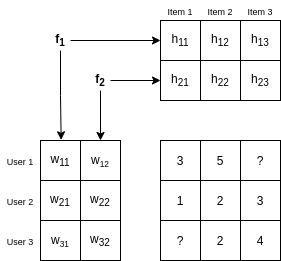
\includegraphics[width=0.5\textwidth]{figures/mf.png}
    \caption{Centralized Matrix Factorization}
    \label{fig:mf}
\end{figure}

\subsection{Decentralized}

In a decentralized context each agent can only access their own data, see Figure \ref{fig:d-mf}. The idea then is to collectively compute the $H$-matrix which is shared between all users, while each agents keeps their own local data as well as their own row of the $W$-matrix.

Given that the $H$-matrix is already computed, each agent has no problem computing $W$ on their own, as they have all the data needed to calculate gradients locally. The challenge is to collectively compute $H$ as each agent only has at most a single data point in the user-movie matrix that can be used to compute a gradient. This results in very noisy gradients. A possible solution could be to make the agents aggregate their gradients before applying them to $H$.

Multiple papers have done decentralized \acrlong{mf}, and although they vary slightly in the type of gradient descent they use, it seems like most used the public-private matrix method. See Section \ref{sec:dezlowrank} to Section \ref{sec:Lin2015} inclusively for these papers. Feel free to look them up. The math used in most of them is quite heavy though, so I have just been sticking to regular gradient descent for now. In my opinion the paper in Section \ref{sec:mishra2016riemannian} seemed pretty promising though.

\begin{figure}
    \centering
    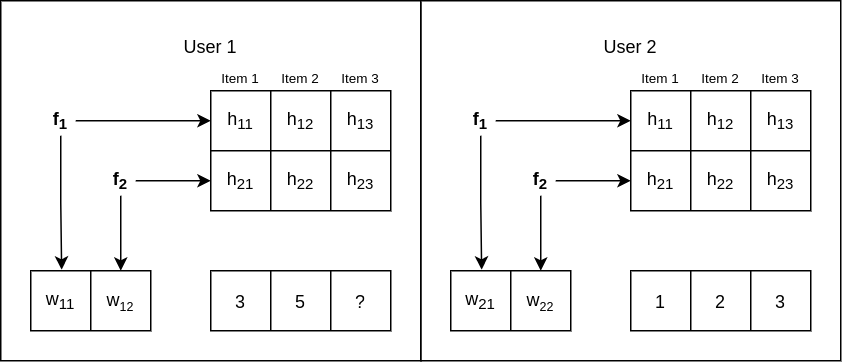
\includegraphics[width=\textwidth]{figures/d-mf.png}
    \caption{Decentralized Matrix Factorization}
    \label{fig:d-mf}
\end{figure}

\section{Decentralized Recommender Systems, \acrlong{fl} and \acrlong{gl}}

\subsection{"Federated Collaborative Filtering for Privacy-Preserving Personalized Recommendation System", \citeyear{ammaduddin2019federated}, \cite{ammaduddin2019federated}}

Introduces a \acrshort{fl}-approach to \acrshort{cf}. Argues that there is a need for a privacy-by-design solution for \acrlongpl{recsys} which does not store users data, while still making users data available for creating robust models. Uses \acrfull{als}. User vectors are calculated locally and not shared. The gradients for the item vector is also calculated locally, but are then aggregated on the central server. Formulated as an implicit feedback \acrshort{mf}-problem, although it is tested on Movielens, an explicit feedback dataset.

\subsection{"Meta Matrix Factorization for Federated Rating Predictions", \citeyear{lin2020meta}, \cite{lin2020meta}}

Uses \acrshort{fl} for users to train a \acrlong{nn} that does rating prediction. Meta-learning is used to create models that are smaller and better suited for mobile devices, the model on the central server is bigger than the models on the mobile devices. Has a central server, but none of the data is shared with the central server. Authors say that user information can be leaked through private item embeddings, RP
models and user updates.

\subsection{"Decentralized Recommendation based on Matrix Factorization: A Comparison of Gossip and Federated Learning", \citeyear{glrecsys}, \cite{glrecsys}}

Introduces a \acrshort{gl}-approach to recommendation systems. Uses \acrshort{sgd} instead of \acrshort{als} due to \acrshort{sgd} being more robust to failure and asynchrony. Vanilla \acrshort{gl} and vanilla \acrshort{fl} does not prevent the receiver of the gradients to try to calculate the users data, but there exists countermeasures for both approaches. Tries to model communication constraints and costs, while also testing the algorithm on the Movielens-dataset. \acrshort{gl} and \acrshort{fl} have similar performance. In general pretty low score on the Movielens-dataset, but this can be because of several reasons. First of all, the authors didn't use the most advanced models, due to it only being a comparison between the two decentralized algorithms. Another reason could be that the realistic modeling of communication restraints lowered performance.

\section{Decentralized Artificial Intelligence}
\subsection{Federated Learning}
\label{sec:federated-learning}

Traditional \acrfull{ml} approaches requires all of the data to be stored on a central machine, but there is a huge amount of data stored on edge devices that could be utilized for training useful \acrshort{ml} models. The owners of this data might not be willing to share it however.

This is why Google introduced \acrfull{fl} \cite{mcmahan2016communicationefficient}

\subsection{Gossip Learning}
\label{sec:federated-learning}

See \cite{gossiplearningalternative}

\subsection{Majority Voting}
\label{sec:mv}

\subsection{Weighted Majority Voting}
\label{sec:wmv}

TODO

\section{Related work}

\section{Market research}

Refer to previous paper?